\documentclass[border=8pt]{standalone}
\usepackage[T1]{fontenc}
\usepackage{mathptmx}
\usepackage{tikz}
\usetikzlibrary{arrows.meta,positioning,fit,calc,shapes.geometric,shapes.misc,shapes.multipart,backgrounds}
\tikzset{
  arr/.style={-{Stealth[length=2.4mm,width=1.8mm]},line width=0.6pt},
  box/.style={draw,line width=0.6pt,align=center,rounded corners=2pt},
}

\begin{document}
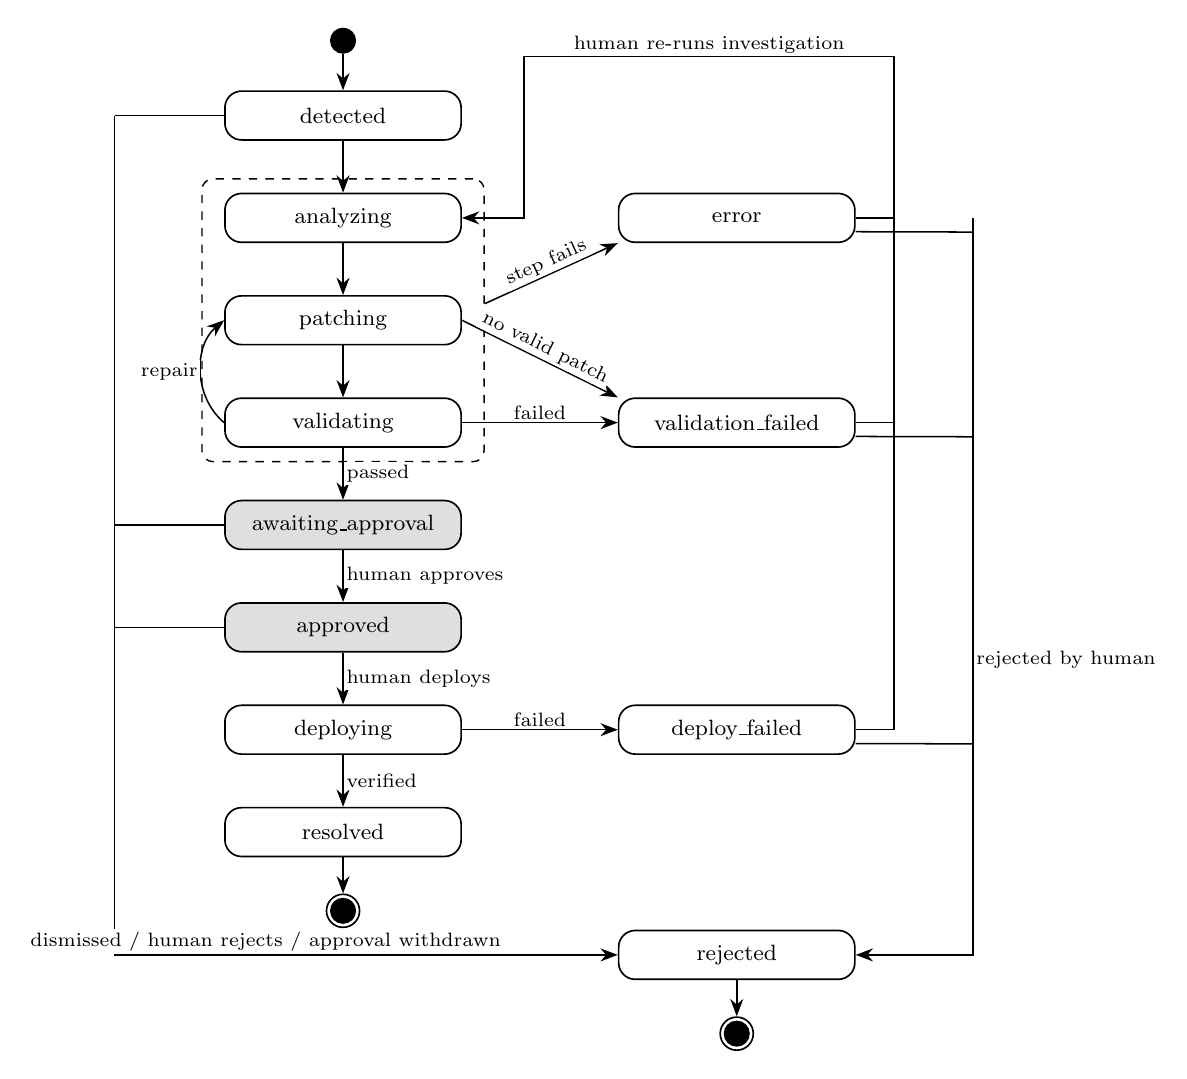
\begin{tikzpicture}[font=\footnotesize,
  st/.style={draw, rounded corners=6pt, line width=0.6pt, minimum width=3.0cm, minimum height=0.62cm, align=center},
  hum/.style={st, fill=gray!25},
  tr/.style={-{Stealth[length=2.2mm]}, line width=0.55pt},
  g/.style={font=\scriptsize, inner sep=1pt, fill=white}]
\def\s{1.3}
\node[circle, fill=black, minimum size=0.32cm] (init) at (0,0.95) {};
\node[st] (det) at (0,0) {detected};
\node[st] (ana) at (0,-1*\s) {analyzing};
\node[st] (pat) at (0,-2*\s) {patching};
\node[st] (val) at (0,-3*\s) {validating};
\node[hum] (wait) at (0,-4*\s) {awaiting\_approval};
\node[hum] (app) at (0,-5*\s) {approved};
\node[st] (dep) at (0,-6*\s) {deploying};
\node[st] (res) at (0,-7*\s) {resolved};
\node[circle, draw, line width=0.6pt, minimum size=0.42cm] (f1) at (0,-7*\s-1.0) {}; \node[circle, fill=black, minimum size=0.26cm] at (f1) {};
\node[st] (err) at (5.0,-1*\s) {error};
\node[st] (vf) at (5.0,-3*\s) {validation\_failed};
\node[st] (df) at (5.0,-6*\s) {deploy\_failed};
\node[st] (rej) at (5.0,-8.2*\s) {rejected};
\node[circle, draw, line width=0.6pt, minimum size=0.42cm] (f2) at (5.0,-8.2*\s-1.0) {}; \node[circle, fill=black, minimum size=0.26cm] at (f2) {};
\begin{scope}[on background layer]\node[draw, dashed, line width=0.5pt, rounded corners=4pt, fit=(ana)(val), inner xsep=8pt, inner ysep=5pt] (grp) {};\end{scope}
\draw[tr] (init)--(det);
\draw[tr] (det)--(ana); \draw[tr] (ana)--(pat); \draw[tr] (pat)--(val);
\draw[tr] (val)--node[g, right]{passed}(wait);
\draw[tr] (wait)--node[g, right]{human approves}(app);
\draw[tr] (app)--node[g, right]{human deploys}(dep);
\draw[tr] (dep)--node[g, right]{verified}(res);
\draw[tr] (res)--(f1);
\draw[tr] (val.west) to[bend left=50] node[g, left]{repair} (pat.west);
% failures
\draw[tr] ([yshift=6pt]grp.east |- pat.east) -- node[g, above, sloped]{step fails} (err.south west);
\draw[tr] (val.east) -- node[g, above]{failed} (vf.west);
\draw[tr] (pat.east) -- node[g, above, sloped]{no valid patch} (vf.north west);
\draw[tr] (dep.east) -- node[g, above]{failed} (df.west);
% human re-run back to analyzing
\draw[line width=0.55pt] (err.east) -- (7.0,-1*\s) (vf.east) -- (7.0,-3*\s) (df.east) -- (7.0,-6*\s);
\draw[tr] (7.0,-6*\s) -- (7.0,0.75) -- node[g, above]{human re-runs investigation} (2.3,0.75) |- (ana.east);
% rejection (terminal)
\draw[line width=0.55pt] (det.west) -- (-2.9,0) (wait.west) -- (-2.9,-4*\s) (app.west) -- (-2.9,-5*\s);
\draw[tr] (-2.9,0) -- (-2.9,-8.2*\s) -- node[g, above, pos=0.3]{dismissed / human rejects / approval withdrawn} (rej.west);

\draw[tr] (8.0,-1*\s) |- node[g, right, pos=0.3]{rejected by human} (rej.east);
\draw[line width=0.55pt] ([yshift=-5pt]err.east) -- (8.0,-1*\s-0.18) ([yshift=-5pt]vf.east) -- (8.0,-3*\s-0.18) ([yshift=-5pt]df.east) -- (8.0,-6*\s-0.18);
\draw[tr] (rej)--(f2);
\end{tikzpicture}
\end{document}
